% Standalone TikZ figure: Summary of Key Contributions
% For Chapter 10: Conclusion and Future Directions
\documentclass[tikz,border=10pt]{standalone}
\usepackage{tikz}
\usetikzlibrary{arrows.meta, positioning, shapes.geometric, fit, backgrounds, calc, decorations.pathreplacing}

\begin{document}
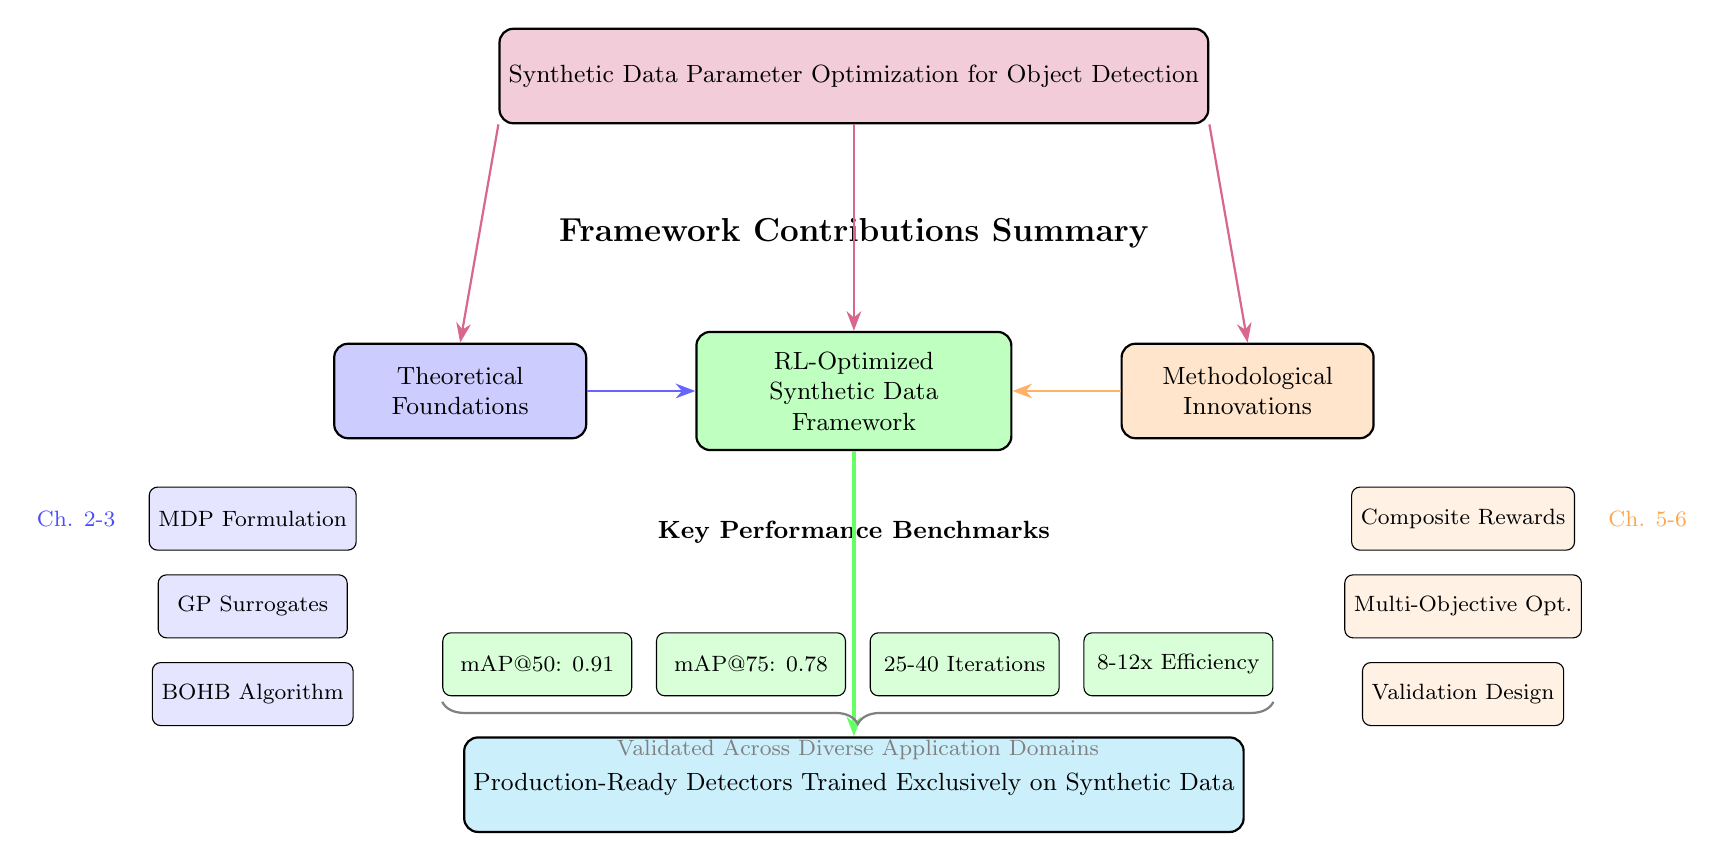
\begin{tikzpicture}[
    node distance=1.0cm and 1.8cm,
    every node/.style={font=\small},
    mainbox/.style={rectangle, draw, thick, minimum width=3.2cm, minimum height=1.2cm, align=center, rounded corners=5pt},
    metricbox/.style={rectangle, draw, minimum width=2.4cm, minimum height=0.8cm, align=center, rounded corners=3pt, font=\footnotesize},
    arrow/.style={-{Stealth[length=2.5mm]}, thick},
    title/.style={font=\bfseries\large},
    subtitle/.style={font=\bfseries\small}
]

% Central title
\node[title] at (0, 2) {Framework Contributions Summary};

% ============ LEFT COLUMN: Theoretical Foundations ============
\node[mainbox, fill=blue!20] (theory) at (-5, 0) {Theoretical\\Foundations};

\node[metricbox, fill=blue!10, below left=0.6cm and -0.3cm of theory] (mdp) {MDP Formulation};
\node[metricbox, fill=blue!10, below=0.3cm of mdp] (gp) {GP Surrogates};
\node[metricbox, fill=blue!10, below=0.3cm of gp] (bohb) {BOHB Algorithm};

% ============ CENTER: Core Framework ============
\node[mainbox, fill=green!25, minimum width=4cm, minimum height=1.5cm] (core) at (0, 0) {RL-Optimized\\Synthetic Data\\Framework};

% Performance metrics below core
\node[subtitle] at (0, -1.8) {Key Performance Benchmarks};

\node[metricbox, fill=green!15, below left=2.3cm and 0.8cm of core] (map50) {mAP@50: 0.91};
\node[metricbox, fill=green!15, right=0.3cm of map50] (map75) {mAP@75: 0.78};
\node[metricbox, fill=green!15, right=0.3cm of map75] (iter) {25-40 Iterations};
\node[metricbox, fill=green!15, right=0.3cm of iter] (eff) {8-12x Efficiency};

% ============ RIGHT COLUMN: Methodological Innovations ============
\node[mainbox, fill=orange!20] (methods) at (5, 0) {Methodological\\Innovations};

\node[metricbox, fill=orange!10, below right=0.6cm and -0.3cm of methods] (reward) {Composite Rewards};
\node[metricbox, fill=orange!10, below=0.3cm of reward] (pareto) {Multi-Objective Opt.};
\node[metricbox, fill=orange!10, below=0.3cm of pareto] (valid) {Validation Design};

% ============ TOP: Problem Domain ============
\node[mainbox, fill=purple!20, minimum width=8cm] (problem) at (0, 4) {Synthetic Data Parameter Optimization for Object Detection};

% ============ BOTTOM: Outcomes ============
\node[mainbox, fill=cyan!20, minimum width=8cm] (outcome) at (0, -5) {Production-Ready Detectors Trained Exclusively on Synthetic Data};

% ============ ARROWS ============
% From problem to components
\draw[arrow, purple!60] (problem.south west) -- (theory.north);
\draw[arrow, purple!60] (problem.south) -- (core.north);
\draw[arrow, purple!60] (problem.south east) -- (methods.north);

% From components to core
\draw[arrow, blue!60] (theory.east) -- (core.west);
\draw[arrow, orange!60] (methods.west) -- (core.east);

% From core to outcome
\draw[arrow, green!60, line width=1.5pt] (core.south) -- ++(0,-1.5) -- (outcome.north);

% Braces for metrics
\draw[decorate, decoration={brace, amplitude=8pt, mirror}, thick, gray]
    ([yshift=-2pt]map50.south west) -- ([yshift=-2pt]eff.south east)
    node[midway, below=10pt, font=\footnotesize, text=gray] {Validated Across Diverse Application Domains};

% Side annotations
\node[font=\footnotesize, text=blue!70, align=center, left=0.3cm of mdp] {Ch. 2-3};
\node[font=\footnotesize, text=orange!70, align=center, right=0.3cm of reward] {Ch. 5-6};

\end{tikzpicture}
\end{document}
